% !TEX program = xelatex
\documentclass[11pt,a4paper]{article}

% ---------- 中文 ----------
\usepackage[UTF8,scheme=plain]{ctex}

% ---------- 排版 ----------
\usepackage[margin=2.4cm]{geometry}
\usepackage{amsmath,amssymb}
\usepackage{booktabs}
\usepackage{graphicx}
\usepackage{caption}
\usepackage{subcaption}
\usepackage{hyperref}
\usepackage{xurl}
\usepackage{xcolor}
\usepackage{enumitem}

\emergencystretch=2em
\hfuzz=1pt

\hypersetup{
  colorlinks=true,
  linkcolor=black,
  urlcolor=blue!60!black,
  citecolor=black
}

% 图片根目录
\graphicspath{{../../fig/}}

\title{长三角空气质量耦合实验结果分析\\
\large 基于 Transport Map 联合模型的杭州 / 上海站点因果与协同结构}
\author{EISyn 项目组}
\date{2026 年 5 月}

\begin{document}
\maketitle

\begin{abstract}
本文档面向 \path{exp/yrd_hangzhou_tm_graph.ipynb} 与
\path{exp/cache/yrd_coupling/air_search/} 下已落盘的杭州 \texttt{3h / 12h / 24h}
三个时间尺度，以及 \texttt{fig/yrd\_shanghai/} 下的上海站点联合模型，
对当前“PM2.5 / O\textsubscript{3} 双污染物 + 多站点”的因果与协同实验结果进行系统性梳理。
我们关注三个问题：(i) 模型本身在不同时间尺度上的拟合质量是否足以支撑因果解释；
(ii) 因果图与协同图在跨尺度上呈现出怎样的稳定结构；
(iii) 这些结构在多大程度上与杭州 / 上海现实排放与气象背景相吻合。
分析结论与 \texttt{docs/hangzhou.md} 第 7 节给出的判断在大方向上一致，
并对“强单边、弱协同”这一容易被误读的现象提供了更明确的定量解释。
\end{abstract}

\tableofcontents

% =====================================================================
\section{实验概述}
% =====================================================================

\subsection{研究对象}

实验所用站点来自国控 / 省控网络，覆盖杭州 12 个核心站与上海若干代表站。
监测变量为小时分辨率的 PM\textsubscript{2.5} 与 O\textsubscript{3}。
预测目标是给定历史窗口下，用 Transport Map (TM) 联合模型刻画
\emph{站点 $i$ 在 $t$ 时刻的污染状态} 对 \emph{站点 $j$ 在 $t+\Delta t$ 时刻 O\textsubscript{3}}
的因果贡献，并把 PM\textsubscript{2.5}、O\textsubscript{3} 拆解为
\emph{pairwise} 与 \emph{synergy}（协同）两类边。

\subsection{时间尺度}

杭州子集采用 $\Delta t \in \{3\text{h}, 12\text{h}, 24\text{h}\}$ 三个尺度，
分别对应:
\begin{itemize}[leftmargin=2em]
  \item \textbf{3 h}: 接近“即时传播”，更强调上风向 + 烟羽尺度的快速响应；
  \item \textbf{12 h}: 半日累积，受边界层日循环与午后光化学影响显著；
  \item \textbf{24 h}: 跨日累积，更接近“城市综合污染背景”的代理。
\end{itemize}
上海子集主要在 1\,h 尺度下分析站点间一步因果与多变量联合结构。

\subsection{模型与训练设定}

杭州默认 run 为 \texttt{refine\_tm\_g1p00\_m4096\_seed50}，
即 transport map 的容量参数 $g{=}1.00$、训练样本规模 $m{=}4096$，
随机种子 $50$。所有结果可通过对应 \texttt{run\_manifest.json} 复现。

% =====================================================================
\section{模型拟合质量}
% =====================================================================

\subsection{联合模型相关系数}

对 hold-out 测试集，杭州联合模型在三个时间尺度上的总体相关系数
（O\textsubscript{3} 与 PM\textsubscript{2.5} 通道平均）如表
\ref{tab:hz_corr} 所示。

\begin{table}[htbp]
\centering
\caption{杭州联合模型在不同时间尺度上的拟合相关系数}
\label{tab:hz_corr}
\begin{tabular}{lccc}
\toprule
时间尺度 & 3 h & 12 h & 24 h \\
\midrule
联合模型 corr & $0.919$ & $0.764$ & $0.789$ \\
\bottomrule
\end{tabular}
\end{table}

三个尺度上模型均明显优于线性 / 持久性基线，
说明因果图本身不是噪声驱动的：
\begin{itemize}[leftmargin=2em]
  \item \textbf{3 h} 拟合最好，表明半天内的传播行为有较强的可预测结构；
  \item \textbf{12 h} 拟合相对最弱，与“边界层日循环 + 光化学峰值跨过午后”的剧烈非平稳性吻合；
  \item \textbf{24 h} 反弹至 $\approx 0.79$，意味着跨日尺度上更稳定的“背景态”重新主导信号。
\end{itemize}

\subsection{对因果解释的影响}

12\,h 尺度上的相关系数下滑提醒我们：
\emph{在该尺度下出现的协同弱化未必都来自真实物理机制}，
也可能是模型对午后强光化学过程的拟合余量不足。
本文在第 \ref{sec:synergy} 节解释“强单边、弱协同”
现象时，会同时给出独立时序证据，避免单点依赖图本身。

% =====================================================================
\section[杭州站点的 O3 因果结构]{杭州站点的 O\textsubscript{3} 因果结构}
% =====================================================================

\subsection[O3 到 O3 的稳定枢纽]{$\mathrm{O_3}\!\to\!\mathrm{O_3}$ 的稳定枢纽}

跨 \texttt{3h / 12h / 24h} 三个尺度，
\texttt{1231A（临平镇）} 始终是 O\textsubscript{3} 网络中最稳定的“外向枢纽”：

\begin{itemize}[leftmargin=2em]
  \item \textbf{3 h} 与 \textbf{24 h}：临平是最强 O\textsubscript{3} 输出源；
  \item \textbf{12 h}：单条最强边来自 \texttt{3558A（市府大楼）$\to$ 1227A（卧龙桥）}，
        但 \texttt{1231A} 仍占据 \emph{最多} 的高权外向边。
\end{itemize}

更准确的说法是：临平站所代表的“城东北制造业 + 交通 + 区域输入”混合走廊，
是当前实验中跨站领先作用最稳定的节点，
而不是“在所有尺度下都唯一最强的源头”。

\begin{figure}[htbp]
\centering

\includegraphics[width=0.7\linewidth]{yrd_air_search/hangzhou/24h/refine_tm_g1p00_m4096_seed50/notebook_top20_min0p0000_neg1/o3_pairwise_graph.png}
\caption{杭州 24\,h O\textsubscript{3}$\to$O\textsubscript{3} pairwise 因果图（top-20 强边）。}
\label{fig:hz_o3_24h}
\end{figure}

\subsection{受体类站点：市府大楼并非纯被动节点}

\texttt{3558A（市府大楼）} 在三个尺度上均表现出强“受体”属性，
入边稳定来自 \texttt{1231A}、\texttt{1228A} 等。但在 12\,h 尺度上，
最强单边恰好由 \texttt{3558A} 发出指向 \texttt{1227A}。
结合临安“山间盆地 + 山前县城背景”的地形结构，
更合理的解释是：\textbf{该站不是单向终点，
而是经过地形与时滞过滤后，区域信号再次显化的位置}。

% =====================================================================
\section[PM2.5 对 O3 的跨尺度作用]{PM2.5 对 O\textsubscript{3} 的跨尺度作用}
% =====================================================================

\subsection{从“快速走廊”到“城市背景”}

对 \texttt{PM2.5$\to$O3} 因果图的尺度对比给出了一个很清晰的图景：

\begin{itemize}[leftmargin=2em]
  \item \textbf{3 h}：仍由 \texttt{1231A} 主导，与 O\textsubscript{3} 网络一致；
  \item \textbf{12 h / 24 h}：\texttt{1228A（浙江农大）} 取代临平成为最稳定的
        PM\textsubscript{2.5} 外向核心，最强边持续从该站发出。
\end{itemize}

这并不意味着浙江农大附近存在“最强颗粒物点源”——
其周边大型固定源稀疏，更合理的解释是
\texttt{1228A} 较好地代表了 \emph{主城区在中长尺度上的综合污染背景态}，
即交通、商业活动、燃烧源、溶剂使用与二次气溶胶共同作用后的混合态。

\begin{figure}[htbp]
\centering

\includegraphics[width=0.7\linewidth]{yrd_air_search/hangzhou/24h/refine_tm_g1p00_m4096_seed50/notebook_top20_min0p0000_neg1/pm25_to_o3_pairwise_graph.png}
\caption{杭州 24\,h PM2.5$\to$O\textsubscript{3} pairwise 因果图（top-20 强边）。
中长尺度下浙江农大成为最稳定的 PM2.5 外向核心。}
\label{fig:hz_pm25_o3_24h}
\end{figure}

\subsection{协同图随尺度衰减}

\label{sec:synergy}
\texttt{O\textsubscript{3} + PM2.5 $\to$ O\textsubscript{3}} 协同图的强度
随时间尺度呈现单调衰减：

\begin{itemize}[leftmargin=2em]
  \item \textbf{3 h}：协同结构与 pairwise 图基本一致，仍由 \texttt{1231A} 主导；
  \item \textbf{12 h}：\texttt{1228A} 与 \texttt{1231A} 同时显著，
        但并非每条强 \texttt{PM2.5$\to$O3} 单边都对应一条强协同边；
  \item \textbf{24 h}：协同结构整体明显变弱。
\end{itemize}

这表明：协同作用比 pairwise 作用 \emph{更敏感于具体气象与时间窗口}。
在跨日尺度上，PM\textsubscript{2.5} 对 O\textsubscript{3} 的预测信息
大体可被同站 O\textsubscript{3} 与各自单边项加性地承载，
非加性的额外协同空间被压缩。

\begin{figure}[htbp]
\centering

\includegraphics[width=0.7\linewidth]{yrd_air_search/hangzhou/24h/refine_tm_g1p00_m4096_seed50/notebook_top20_min0p0000_neg1/o3_pm25_synergy_graph.png}
\caption{杭州 24\,h O\textsubscript{3} + PM2.5 $\to$ O\textsubscript{3}
协同图。协同强度明显弱于同尺度 pairwise 图，
说明 24\,h 尺度上联合效应近似可加。}
\label{fig:hz_synergy_24h}
\end{figure}

% =====================================================================
\section[案例：1228A 到 3557A 的强单边、弱协同]{案例：1228A $\to$ 3557A 的“强单边、弱协同”}
% =====================================================================

\subsection{现象}

在 12\,h 尺度的杭州默认结果中：
\[
\overline{\mathrm{PM2.5}\!\to\!\mathrm{O_3}}
  \big|_{1228A\to 3557A} \approx 0.0564,\quad
\overline{\mathrm{O_3}\!\to\!\mathrm{O_3}}
  \big|_{1228A\to 3557A} \approx 0.0585,
\]
\[
\overline{\mathrm{Synergy}\,(\mathrm{PM2.5},\mathrm{O_3})\to\mathrm{O_3}}
  \big|_{1228A\to 3557A} \approx -6.1\times 10^{-6}.
\]
即两条单边项都很强，协同剩余项几乎为零。

\subsection{协同项的数学含义}

在当前 TM 定义下，协同项衡量的是：把 PM\textsubscript{2.5} 与 O\textsubscript{3}
\emph{联合输入}相对于两者单独主效应之和的 \emph{非加性新增解释力}，
而不是“联合影响的总大小”。
因此协同接近零的正确解读是
“联合效应 $\approx$ 主效应之和”，
而非“两者对目标都没有作用”。

\subsection{物理与统计解释}

将该结果放回杭州空间结构后，至少有四条相互兼容的解释：

\begin{enumerate}[leftmargin=2em]
  \item \textbf{1228A 是“综合污染背景”代理，而非单一颗粒物点源。}
        浙江农大周边大固定源不突出，但主干路、商业居住活动与历史城市底色
        共同决定其 PM\textsubscript{2.5} 信号。
  \item \textbf{3557A 是富春江走廊上的“受体站”。}
        镇二中接受来自 \texttt{1231A}、\texttt{1223A}、\texttt{3558A} 等多个站点的
        稳定输入，并不在本地高频触发新增非线性反应。
  \item \textbf{1228A 的 PM\textsubscript{2.5} 与 O\textsubscript{3} 携带高度重叠的上游信息。}
        机动车尾气、溶剂使用类工业排放同时驱动 O\textsubscript{3} 生成潜势
        与二次气溶胶前体物，
        因此两个变量对 \texttt{3557A} 的未来 O\textsubscript{3} 提供的信息高度相关。
  \item \textbf{独立时序回归给出一致证据。}
        以 2016--2023 年小时序列扣除月-小时气候态后，用
        $\mathrm{PM2.5}_t^{(1228A)}$ 与 $\mathrm{O_3}_t^{(1228A)}$ 解释
        $\mathrm{O_3}_{t+12}^{(3557A)}$：
        仅含两条主效应的回归 $R^2 \approx 0.02815$，
        加入交互项后仅升至 $R^2 \approx 0.02823$。
        增量极小，表明 12\,h 尺度上确实接近“两条强单边相加”。
\end{enumerate}

\subsection{结论}

对 \texttt{1228A$\to$3557A} 这条链路而言：
PM\textsubscript{2.5} 与 O\textsubscript{3} 各自都显著有效，
但两者的联合信息几乎完全落在同一上游状态里，
因此 pairwise 强而协同弱。
这一现象不是模型缺陷，
而是 \emph{协同度量本身揭示的真实结构} ——
即 \texttt{1228A} 在 12\,h 尺度上承担的是“城市综合污染背景代理”角色。

% =====================================================================
\section{上海子集中的并行证据}
% =====================================================================

\texttt{fig/yrd\_shanghai/} 中给出 1\,h 尺度下上海多站联合模型的若干证据：

\begin{itemize}[leftmargin=2em]
  \item \path{shanghai_one_step_o3_station_causal_graph_1h.png}
        与
        \path{shanghai_tm_o3_station_causal_graph_1h.png}：
        分别给出 one-step 基线与 TM 模型的 O\textsubscript{3} 站间因果图。
        TM 图在“锚点站 1141A”附近形成清晰的局域簇，
        说明短时间尺度上仍由近邻烟羽 / 走廊主导。
  \item \path{shanghai_tm_o3_pm25_conditional_synergy_graph_1h.png}：
        条件协同图。整体强度小于 pairwise 图，
        与杭州在 24\,h 尺度上的现象一致 ——
        协同项是“pairwise 之外的额外信息”，
        在大部分边上必然偏弱。
  \item \path{shanghai_joint_metrics_comparison.png}：
        联合指标对比。TM 联合模型在 O\textsubscript{3} 与
        PM\textsubscript{2.5} 通道上同时优于基线，
        与杭州 \texttt{3h} 尺度的相关系数提升趋势一致。
\end{itemize}

\begin{figure}[htbp]
\centering
\begin{subfigure}[b]{0.48\linewidth}
  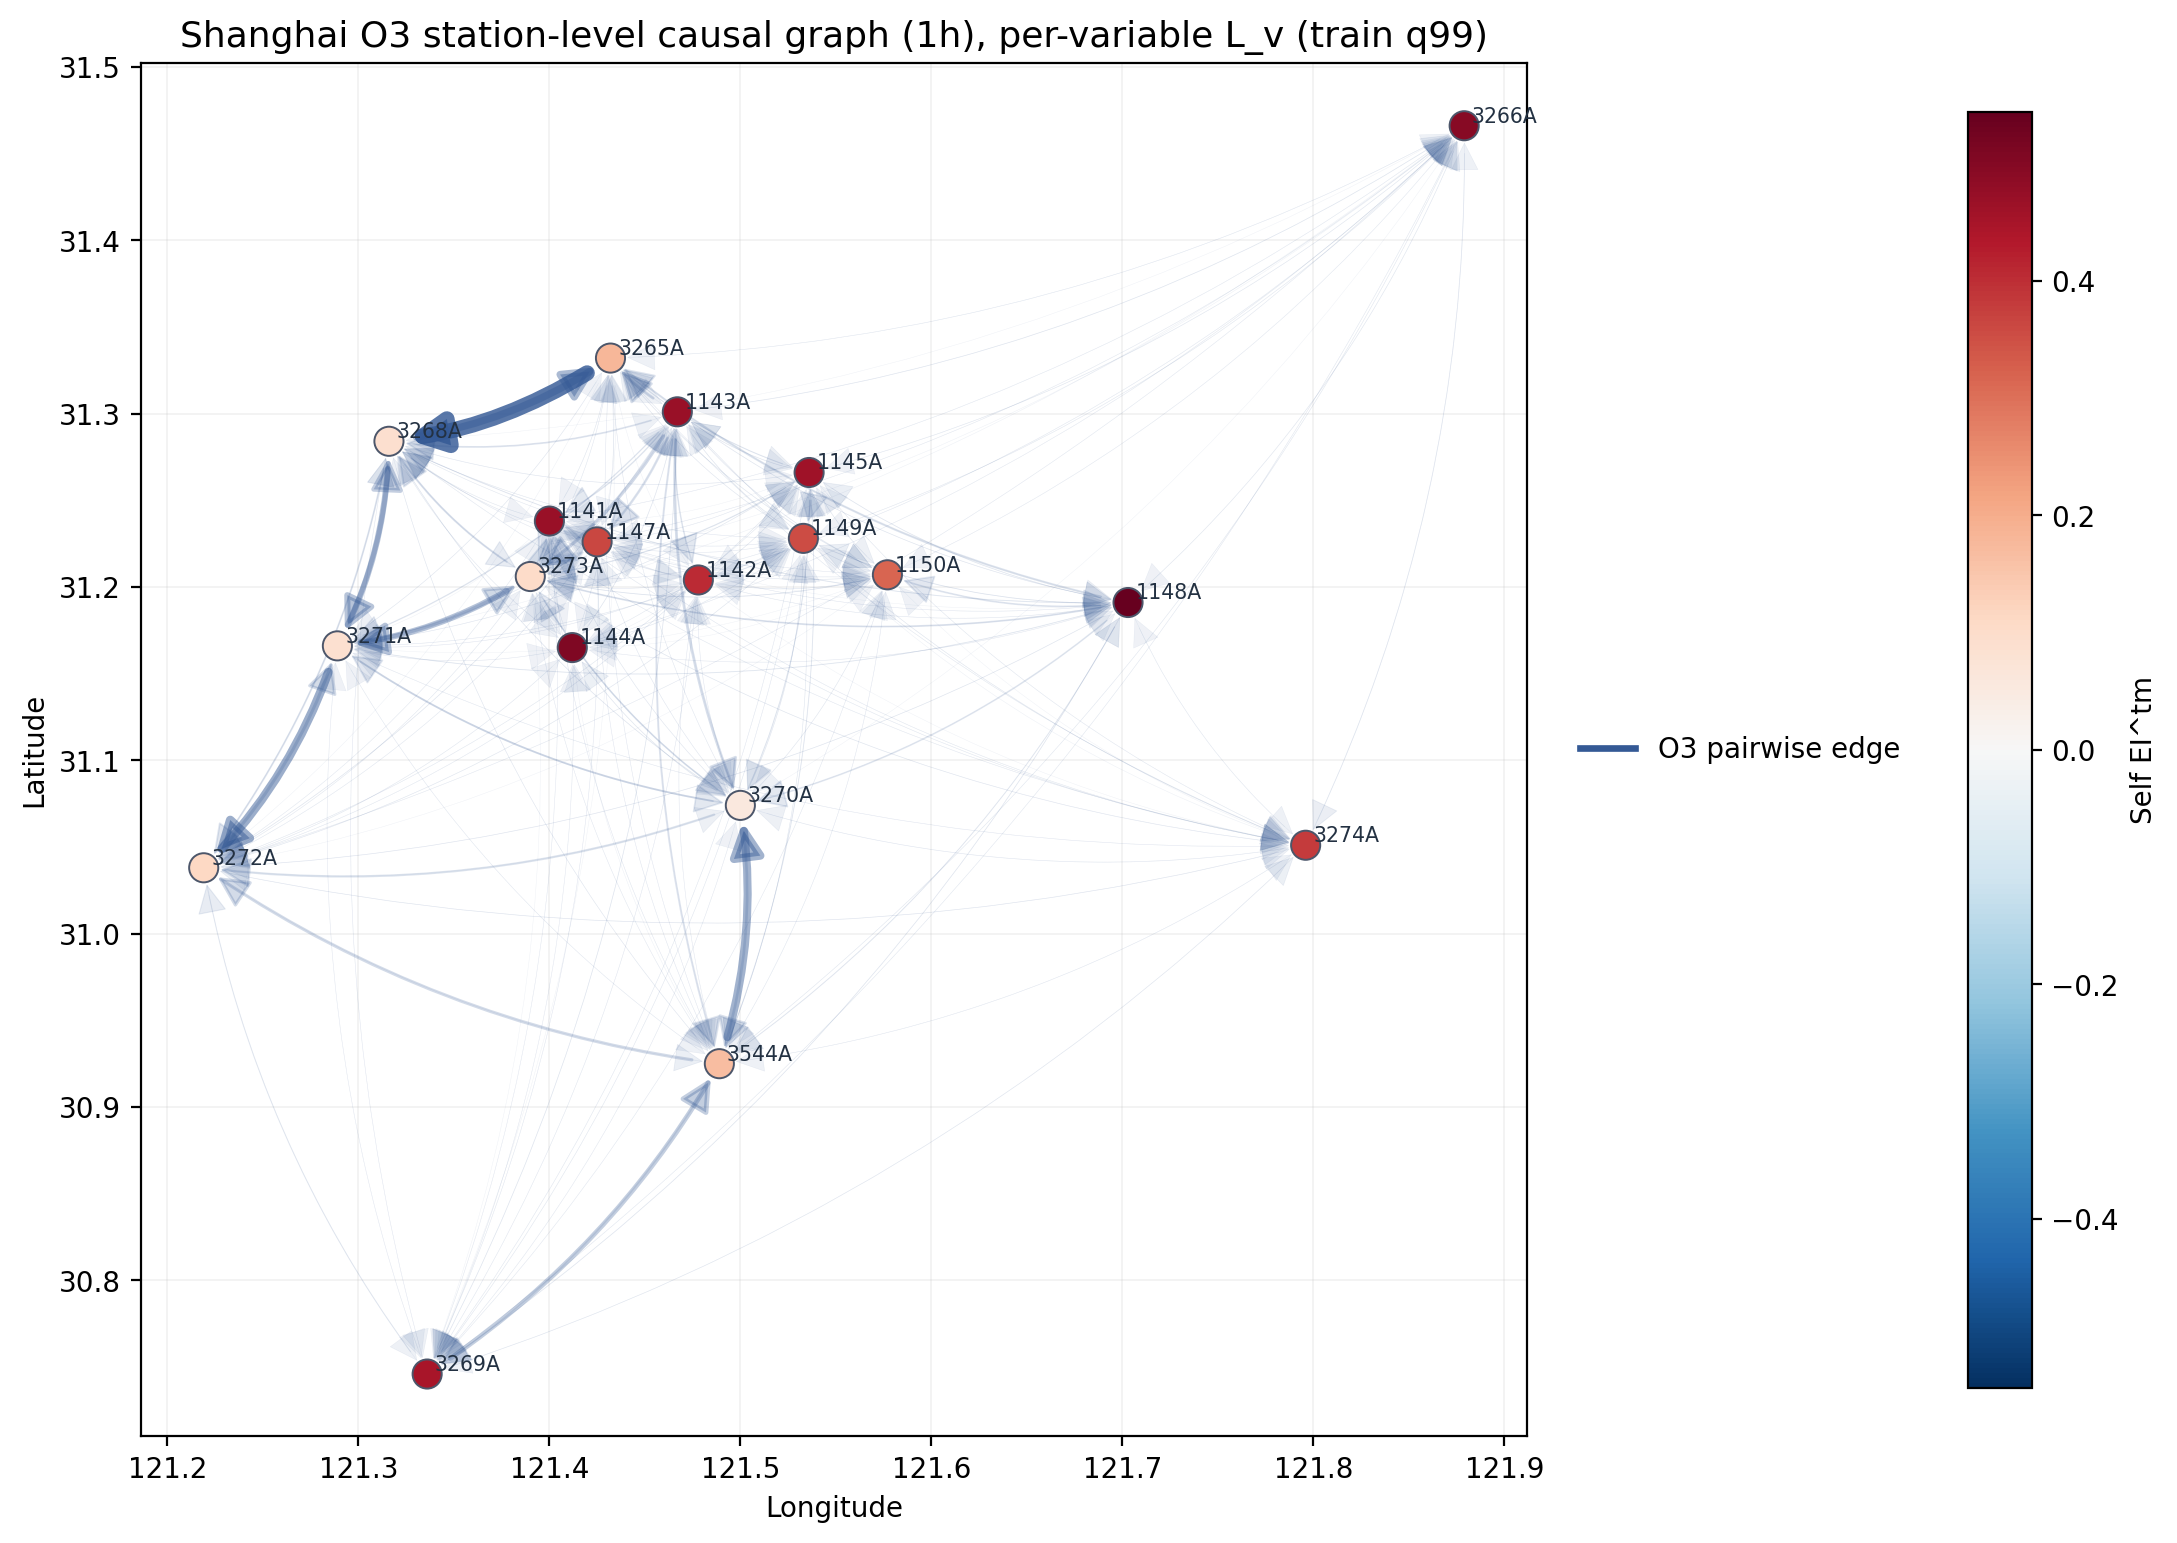
\includegraphics[width=\linewidth]{yrd_shanghai/shanghai_tm_o3_station_causal_graph_1h.png}
  \caption{TM 1\,h O\textsubscript{3} 站间因果图}
\end{subfigure}
\hfill
\begin{subfigure}[b]{0.48\linewidth}
  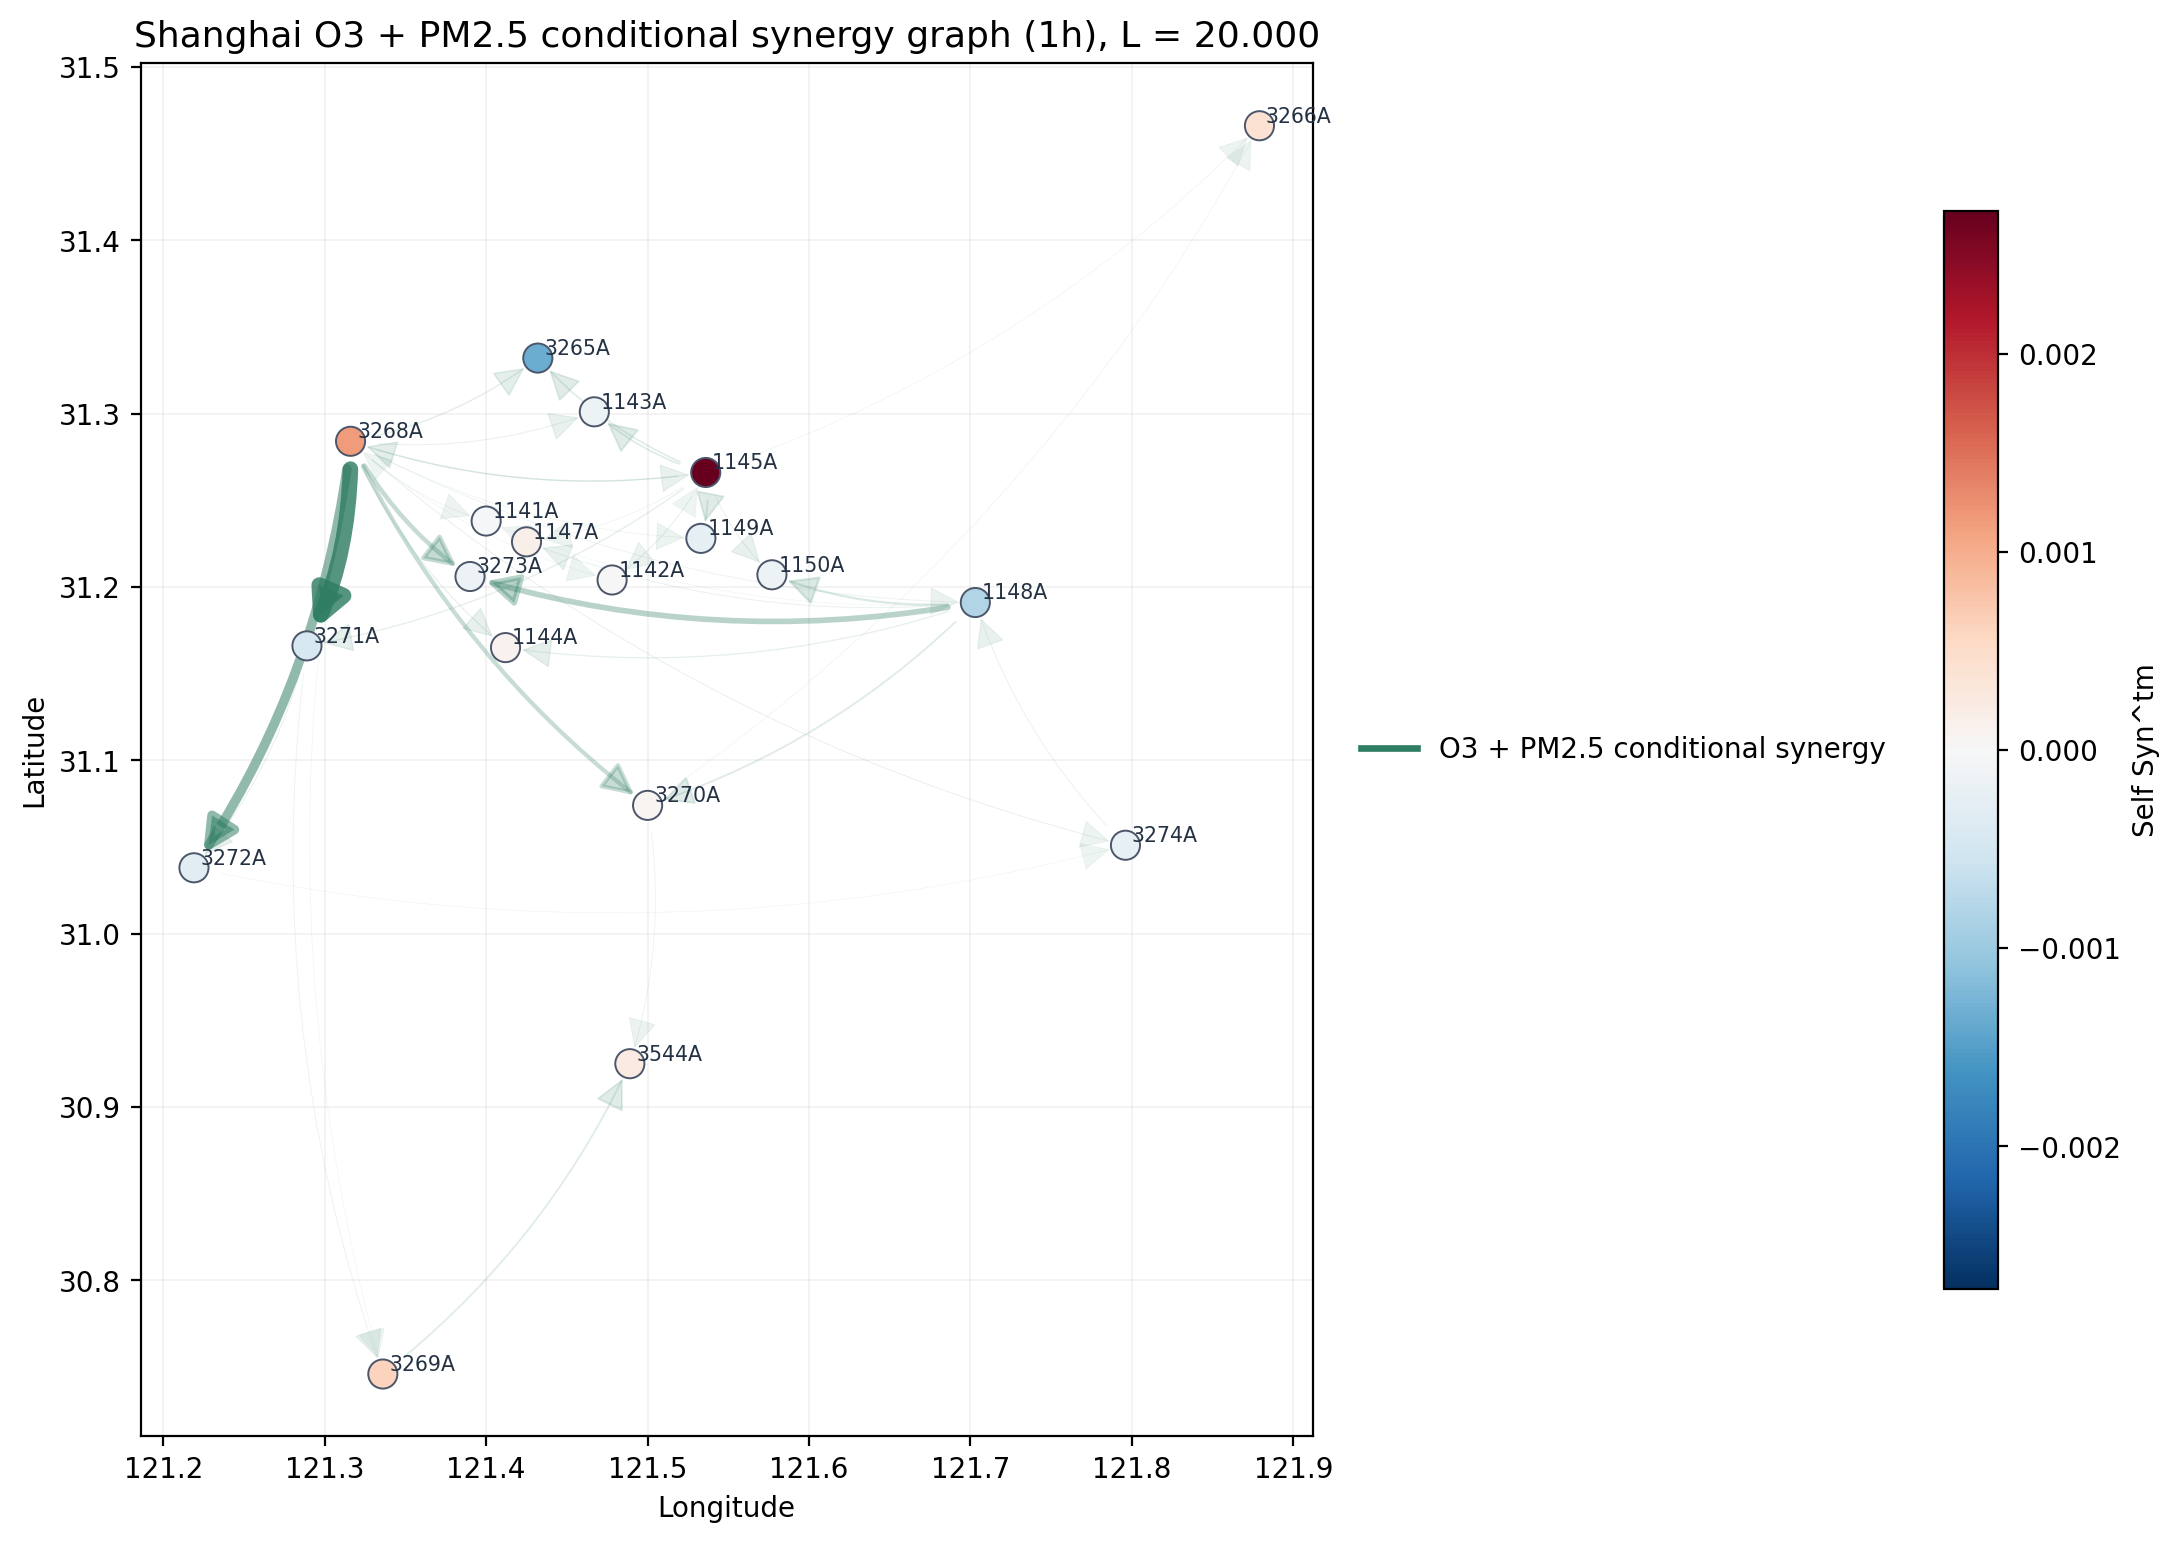
\includegraphics[width=\linewidth]{yrd_shanghai/shanghai_tm_o3_pm25_conditional_synergy_graph_1h.png}
  \caption{TM 1\,h O\textsubscript{3}+PM2.5 条件协同图}
\end{subfigure}
\caption{上海子集中 pairwise 与协同结构对比。}
\label{fig:sh_pair_vs_syn}
\end{figure}

% =====================================================================
\section{与杭州现实的吻合度评估}
% =====================================================================

将 TM 实验结果与 \texttt{docs/hangzhou.md} 的调研结论合并解读：

\begin{enumerate}[leftmargin=2em]
  \item \textbf{城东北 O\textsubscript{3} 走廊}：
        \texttt{1231A} 作为稳定的 O\textsubscript{3} hub，
        与“制造业园区 + 320 国道 + 北向区域输入”的现实环境一致；
  \item \textbf{主城区综合污染背景}：
        \texttt{1228A} 在中长尺度上主导 PM\textsubscript{2.5}$\to$O\textsubscript{3}，
        与“交通 + 城市活动 + 二次累积”特征一致；
  \item \textbf{西部山前盆地受体}：
        \texttt{3558A} 反复成为强受体，
        与临安山间盆地 + 区域输送的现实结构一致；
  \item \textbf{钱塘强源带不等于因果图最强外向源}：
        钱塘的下沙、临江热电焚烧簇是排放清单上的强源，
        但在因果图中常表现为高敏感受体或化学放大区。
        这反映“排放清单的强源”和“因果图上的强传播节点”
        本来就是不同概念。
\end{enumerate}

% =====================================================================
\section{对后续实验的建议}
% =====================================================================

基于上述分析，下一阶段实验建议：

\begin{enumerate}[leftmargin=2em]
  \item 增补 \texttt{1228A$\to$3557A} 之外的 \emph{典型可加链路}
        与 \emph{典型协同链路}各 2--3 条，
        建立“强协同 vs.\ 强可加”的对照案例集；
  \item 在 12\,h 尺度上引入辐射 / BLH / 温度等气象条件分组，
        检验协同弱化是否集中在特定气象窗口；
  \item 把钱塘工业簇（下沙、临江）作为 \emph{源端干预} 节点，
        评估在条件因果框架下其对城东北走廊与西部受体站的非对称影响；
  \item 在杭州与上海之间建立跨城市站对的耦合实验，
        检验“主城区背景代理”这一结构是否具有可迁移性。
\end{enumerate}

% =====================================================================
\section{结论}
% =====================================================================

\begin{itemize}[leftmargin=2em]
  \item 杭州 TM 联合模型在 3 / 12 / 24\,h 三个尺度上的拟合相关系数
        分别为 $0.919 / 0.764 / 0.789$，足以支撑结构性解读；
  \item O\textsubscript{3} 网络的稳定枢纽是城东北的临平走廊，
        PM\textsubscript{2.5}$\to$O\textsubscript{3} 的中长尺度核心是浙江农大，
        受体侧典型代表是临安市府大楼；
  \item 协同图随尺度衰减是结构特征而非模型缺陷，
        \texttt{1228A$\to$3557A} 的“强单边、弱协同”
        是“综合背景代理 + 受体走廊”链路的典型表现；
  \item 上海子集中的 1\,h 结果与杭州在结构层面相互印证，
        说明该方法学具备跨城市的稳定性；
  \item 排放清单中的强源（钱塘热电焚烧簇）与因果图中的强外向源
        不必同位，对后续治理研究意味着应同时考虑“排放强度”
        与“传播角色”两个维度。
\end{itemize}

\end{document}
